% IF YOU CAN SEE THIS GO CONTRIBUTE >:(

\documentclass[letterpaper, 8pt]{extarticle}
\usepackage{amssymb,amsmath,amsthm,amsfonts}
\usepackage{multicol,multirow}
\usepackage{calc}
\usepackage{ifthen}
\usepackage[landscape]{geometry}
\usepackage[colorlinks=true,citecolor=blue,linkcolor=blue]{hyperref}

\usepackage{booktabs}
\usepackage{ulem}
\usepackage{enumitem}
\usepackage{tabulary}
\usepackage{graphicx}
\usepackage{siunitx}
\usepackage{tikz}
\usepackage{derivative}
\usepackage{svg}
\usepackage{listings}
\usepackage{setspace}
\usepackage{listings}
\usepackage{xcolor}
\usepackage{courier}
\usepackage{syntax}
\usepackage{mathpartir}

% minimal line spacing
% NOTE: this makes math look bad, only use as a last resort
% \setstretch{0.1}

% set borders (experimentally determined to minimize cutoff and maximize space on school printers)
% NOTE: if you wish to tune this, please only do so on your local copy
\geometry{top=.25in,left=.25in,right=.25in,bottom=.35in}

% make figures work better in multicol
\newenvironment{Figure}
{\par\medskip\noindent\minipage}
{\endminipage\par\medskip}

\pagestyle{empty} % clear page

% rewrite section commands to be smaller
\makeatletter
\renewcommand{\section}{\@startsection{section}{1}{0mm}%
	{-1explus -.5ex minus -.2ex}%
	{0.5ex plus .2ex}%x
	{\normalfont\normalsize\bfseries}}
\renewcommand{\subsection}{\@startsection{subsection}{2}{0mm}%
	{-1explus -.5ex minus -.2ex}%
	{0.5ex plus .2ex}%
	{\normalfont\small\bfseries}}
\renewcommand{\subsubsection}{\@startsection{subsubsection}{3}{0mm}%
	{-1ex plus -.5ex minus -.2ex}%
	{1ex plus .2ex}%
	{\normalfont\tiny\bfseries}}
\makeatother
\setcounter{secnumdepth}{0} % disable section numbering


% disable indenting
\setlength{\parindent}{0pt}
\setlength{\parskip}{0pt plus 0.5ex}

% Custom siunitx defs
\DeclareSIUnit\noop{\relax}
\NewDocumentCommand\prefixvalue{m}{%
	\qty[prefix-mode=extract-exponent,print-unity-mantissa=false]{1}{#1\noop}
}

% Shorthand definitions
\newcommand{\To}{\Rightarrow}
\newcommand{\ttt}{\texttt}
\newcommand{\ra}{\rightarrow}

% condense itemize & enumerate
\let\olditemize=\itemize \let\endolditemize=\enditemize \renewenvironment{itemize}{\olditemize \itemsep0em}{\endolditemize}
\let\oldenumerate=\enumerate \let\endoldenumerate=\endenumerate \renewenvironment{enumerate}{\oldenumerate \itemsep0em}{\endoldenumerate}
\setlist[itemize]{noitemsep, topsep=0pt, leftmargin=*}
\setlist[enumerate]{noitemsep, topsep=0pt, leftmargin=*}

% TODO: CHANGEME
\title{ClassCode}

\begin{document}
\raggedright
\tiny

% make listings look nicer
\lstset{
	tabsize = 2, %% set tab space width
	showstringspaces = false, %% prevent space marking in strings, string is generally printed directly to the console
	basicstyle = \tiny\ttfamily, %% set listing font and size
	breaklines = true, %% enable line breaking
	numberstyle = \tiny,
	postbreak = \mbox{\textcolor{red}{\(\hookrightarrow\)}\space}
}

\begin{center}
	% TODO: CHANGEME
	{\textbf{Graph Theory Cheat Sheet}} \\
\end{center}
% set column spacing rules
\setlength{\premulticols}{1pt}
\setlength{\postmulticols}{1pt}
\setlength{\multicolsep}{1pt}
\setlength{\columnsep}{2pt}

% NOTE: tweak this based on desired content density / readability
\begin{multicols*}{4}
	\section{Fundamental Definitions}
	\textbf{Order/Size}: Order $|V|$, Size $|E|$ (number of edges). \\
	\textbf{Walk}: Alternating sequence of vertices/edges $A_1, e_1, A_2, \dots$ where $e_i$ is incident to $A_{i-1}, A_i$. \\
	\textbf{Open/Closed walk}: Open if $A_1 \ne A_n$; closed if $A_1 = A_n$ (it's a cycle). Length = number of edges. \\
	\textbf{Trail}: A walk with no repeated edges. \\
	\textbf{Closed Trail/Circuit}: A trail where endpoints are the same vertex. \\
	\textbf{Path}: A trail where no vertex is repeated (except potentially endpoints in cycle). \\
	\textbf{Closed Path}: A path whose endpoints are the same vertex. \\
	\textbf{Loop}: a self loop (cycle of length 1). Loops count twice when counting degrees.\\
	\textbf{Lune}: cycle of length 2 \\
	\textbf{Cycle}: A path whose endpoints are the same. Graphs are at least 3 cycles. Pseudographs can have a length 1 or 2 cycle, called a loop or loon. \\
	\textbf{Distance} $d(x,y)$: Length of shortest path. \\
	\textbf{Diameter}: Length of longest shortest path. \\
	\textbf{Bridge}: An edge whose removal disconnects $G$; the two resulting subgraphs are called the \textbf{banks} of the bridge.
	\textbf{Decomposition}: $G$ is decomposable into $H_1, \dots, H_t$ if $H_i$ and $H_j$ have no edges in common and $\bigcup H_i = G$. \\
	\textbf{Girth}: Length of shortest cycle. \\

	\section{Degrees}
	\textbf{Degree} $\deg v$: Number of edges incident to $v$ ($v \in V$). Loops count twice when counting degrees. \\
	\textbf{Isolated}: $\deg v = 0$. \\
	\textbf{End vertex}: $\deg v = 1$. \\
	\textbf{Handshaking Theorem}: For $v_1, \dots, v_n \in V$ and $q$ edges, $\sum_{i=1}^n \deg v_i = 2q$. \\
	\textbf{Degree sequence}: Ordering of degrees in non-decreasing order. \\
	\textbf{Graphic}: Sequence $d_1, \dots, d_p$ is graphic if $\exists G$ with that degree sequence. \\
	\textbf{Havel-Hakimi Theorem}: Consider the following two sequences and assume sequence (1) is in descending order.
	\vspace{-8pt}
	\begin{align}
		s,\  & t_1,\, t_2, \ldots,\, t_s,\, d_1,\, \ldots,\, d_n         \\
		     & t_1-1,\, t_2-1,\, \ldots,\, t_s-1,\, d_1,\, \ldots,\, d_n
	\end{align}
	\vspace{-12pt} \\
	Then sequence (1) is graphic iff sequence (2) is graphic.

	\section{Trees}
	\textbf{Definition}: A connected graph is a \textbf{tree} iff it is acyclic. \\
	\textbf{Forest}: A graph without cycles (collection of trees). \\
	\textbf{Properties}: $G$ is a tree iff:
	\begin{enumerate}
		\item $|V| = |E| + 1$
		\item There exists exactly one path between 2 vertices.
	\end{enumerate}
	\textbf{Bridges theorem}: Every edge of a tree is a bridge. $G$ is a tree iff $G$ is connected and every edge is a bridge.

	\section{Connected Graphs}
	\textbf{Connected}: $G$ is connected if for every pair of vertices $i$ and $j$ there exists a path between $i$ and $j$. \\
	\textbf{Theorem}: If $G$ is connected, then $|V| \le |E| + 1$. \\
	\textbf{Theorem 2.4.2.}: A connected graph with an even number of edges is decomposable into subgraphs each isomorphic to a path of length two.

	\section{Cubic Graphs}
	\textbf{Definition}: A graph where every vertex has degree 3 (3-regular). \\
	\textbf{$Q_n$}: has $2^n$ vertices and a diamter of $n$. Basically $Q_2$ is a square, $Q_3$ is a cube, etc.\\
	\textbf{Decomposition}: If $G$ is cubic, then $G$ has no decomposition into subgraphs, each of which is isomorphic to a path of length four. \\
	\textbf{Bridges}: A cubic graph with a bridge cannot be decomposed into three 1-factors. \\
	\textbf{Petersen's Theorem}: A cubic bridgeless graph $G$ has a decomposition into a 1-factor and a 2-factor. It is also decomposable into paths of length 3.

	\section{Hamiltonian \& Eulerian}
	\textbf{Eulerian Circuit}: Circuit containing every edge of $G$.
	\textbf{Theorem}: Pseudograph $G$ has Eulerian circuit iff $G$ is connected and degree of every vertex is even. \\
	\textbf{Eulerian Trail}: Trail containing every edge/vertex.
	\textbf{Theorem 3.1.6}: Eurlerian trail exists iff $G$ is connected and has precisely two vertices of odd degree. \\
	\textbf{Eulerian line}: An Eulerian Circuit in an infinite lattice graph. A trail containg every edge and vertex with no beginning vertex or ending vertex.
	\textbf{One-way Eurlerian trail}: Exists in an infinite lattice graph with one endpoint and includes every edge exactly once. Starting vertex has odd degree and everything else has even degree. \\
	\textbf{Hamiltonian Cycle}: Cycle containing every vertex. \\
	\textbf{Hamiltonian Path}: Path containing every vertex. \\
	\textbf{Hamilton line}: A Hamilton cycle in an infinite lattice graph. It is a connected 2-factor that's spanning path without an end. \\
	\textbf{One-way Hamiltonian path}: Exists in an infinite lattice graph and starts at $z$ and has an infinite length and passes through every vertex of the graph. \\
	\textbf{Theorem 2.3.1: $K_{2n+1}$} has a decomposition into $n$ Hamiltonian cycles (cannot have all Hamilton cycles for $K_{2n}$). \\
	\textbf{Theorem 2.3.2 and 2.3.3: $K_{2n}$} decomposable into $n-1$ Hamilton cycles and a 1-factor, or into $n$ Hamilton paths. \\
	\textbf{Theorem 2.3.4: $K_{2n}$} has a decomposition into $2n-1$ regular paths consistent of one path of each length $k$ for $k = 1, 2, 3, \dots, 2n-1$. \\
	\textbf{Theorem 2.3.5:} Snarks have no hamiltonian cycle.

	\section{Bipartite Graphs}
	\textbf{Bipartite}: $K_n$ $n$ vertices and every vertex is adjacent to every other vertex. So $K_n$ has $n \choose 2$ edges. \\
	\textbf{Theorem}: $G$ is bipartite iff every cycle has even length or $\chi(G) \le 2$. \\
	\textbf{Complete Bipartite}: $K_{m,n}$ all vertices in a group of $m$ are adjacent to all vertices of a graph with $n$. \\
	\textbf{$k$-partite graph}: a graph where the vertices are partitioned into $k$ sets, and no two vertices in the same set are adjacent. \\

	\section{Vertex Coloring}
	\textbf{Vertex Coloring}: Assignment of colors to vertices s.t. adjacent vertices receive different colours. \\
	\textbf{Chromatic Number} $\chi(G)$: Least number of colours needed to colour $G$. \\
	\textbf{Strategy to prove $\chi(G) = k$}: (1) Find a $k$-colouring. (2) Prove colouring with $\le k-1$ colours is impossible. \\
	\textbf{Critical}: $G$ is critical if $\chi(H) < \chi(G)$ for all proper subgraphs $H$ of $G$. \\
	\textbf{Theorem}: Every graph $G$ has a critical subgraph $H$ s.t. $\chi(H) = \chi(G)$. \\
	\textbf{Theorem}: If $G$ is critical, then $\forall v \in V$, $\deg v \ge \chi(G) - 1$. \\
	\textbf{Theorem}: If $G$ is critical, then $(\chi(G) - 1)|V| \le 2|E|$. \\
	\textbf{Theorem 4.1.1}: The largest graph with $n$ vertices and chromatic number $k$ is a complete $k$-partite graph $K_{n_1, n_2, \ldots, n_k}$ with $n = n_1 + n_2 + \cdots + n_k$ and $|n_i - n_j| \le 1$. \\
	\textbf{Theorem 4.1.2 (Turan)}: The largest graph with $n$ vertices that contains no subgraph isomorphic to $K_{k+1}$ is a complete $k$-partite graph $K_{n_1, n_2, \ldots, n_k}$ with $n = n_1 + n_2 + \cdots + n_k$ and $|n_i - n_j| \le 1$. \\
	\textbf{Theorem 4.1.2$^*$}: The largest graph with $n$ vertices that contains no triangle is the complete bipartite graph $K_{n_1, n_2}$ with $n = n_1 + n_2$ and $|n_1 - n_2| \le 1$. (special case of Turan where $k = 2$) \\
	\textbf{Lemma 4.1.3}: If $G$ is a graph on $n$ vertices that contains no $K_{k+1}$, then there is a $k$-partite graph $H$ with the same vertex set as $G$ such that $\deg_G(z) \le \deg_H(z)$ for every vertex $z$ of $G$.

	\section{Edge Coloring}
	\textbf{Proper Edge Coloring}: Assignment of colors to edges of $G$ s.t. adjacent edges receive unequal colors. \\
	\textbf{Edge Chromatic Number} Smallest number of colors needed for proper edge coloring. \\
	\textbf{$k$-Factor}: A $k$-regular spanning subgraph where every vertex has degree $k$. \\
	\textbf{Theorem}: $k$-regular graphs have an edge chromatic number of $k$ or $k-1$. \\
	\textbf{Theorem}: The edge chromatic number $\ge$ the maximum degree of any vertex of $G$. \\
	\textbf{Theorem}: Edge chromatic number of $K_{2n} = 2n-1$. \\
	\textbf{Theorem}: Edge chromatic number of $K_{2n-1} = 2n-1$. \\
	\textbf{Ramsey $R(m,n)$} (often $r(m,n)$): Least $N$ such that every red/blue edge-coloring of $K_N$ has a red $K_m$ or a blue $K_n$. (Finite for all $m,n\ge 2$.) $R(m,n)=R(n,m)$, $R(2,n)=n$. \textbf{Diagonal} $R(n)=R(n,n)$. \\
	\textbf{Recurrence}: $R(m,n)\le R(m-1,n)+R(m,n-1)$. If $R(m-1,n)$ and $R(m,n-1)$ are both even, then $R(m,n)\le R(m-1,n)+R(m,n-1)-1$. \\
	\textbf{Small values}: $r(1,n) = 1$, $r(2,n) = n$, $R(3,3)=6$, $R(3,4)=9$, $R(3,5)=14$, $R(3,6)=18$, $R(3,7)=23$, $R(3,8)=28$, $R(3,9)=36$; $R(4,4)=18$, $R(4,5)=25$, $R(4,6)=41$. \\
	\textbf{Diagonal}: $R(3)=6$, $R(4)=18$; $R(5)$ unknown, $43\le R(5)\le 48$. \\

	\section{Multigraphs \& Pseudographs}
	\textbf{Multigraph}: Allows multiple edges between vertices. \\
	\textbf{Pseudograph}: Allows multiple edges and self-loops. \\
	\textbf{Eulerian Circuit}: Trail containing every edge in $G$. \\
	\textbf{Theorem 3.1.1}: If pseudograph $G$ has eulerian circuit, then $G$ is connected and the degree of every vertex is even. \\
	\textbf{Theorem 3.1.2}: If a pseudograph $G$ is connected, and the degree of every vertex of $G$ is even, then $G$ has an eulerian circuit. \\
	\textbf{Theorem 3.1.3}: If every vertex in a pseudograph $G$ has positive even degree, then any given vertex of $G$ lies on some circuit of $G$. \\
	\textbf{Theorem 3.1.4}: If a pseudograph $G$ is regular of degree 4, then $G$ has a decomposition into two 2-factors. \\
	\textbf{Theorem 3.1.5}: Pseudograph $G$ has a decomposition into cycles iff every vertex of $G$ has even degree. \\
	\textbf{Theorem 3.1.6}: Pseudograph $G$ has an eulerian trail iff $G$ is connected and has precisely two vertex of odd degree. \\
	\textbf{Theorem 3.1.7}: If $G$ is connected pseudograph with precisely 2h vertex of odd degree, $h \ne 0$, then there exists $h$ trails in $G$ s.t. each edge of $G$ is in exactly one of these trails. Furthermore, fewwer than $h$ trails with this property cannot be found. \\

	\section{Special Graphs}
	\textbf{Petersen Graph}: The unique 5-cage; cubic bridgeless. Decomposes into a 1-factor and a 2-factor. \\
	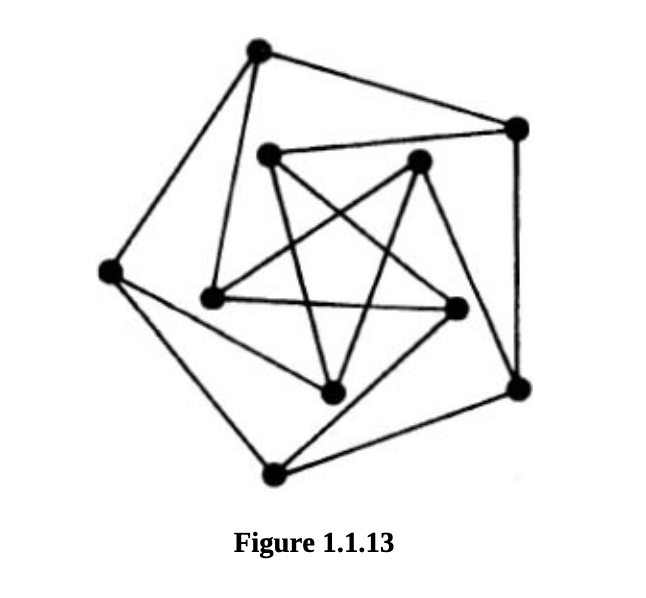
\includegraphics[width=0.25\linewidth]{petersen-graph.png}
	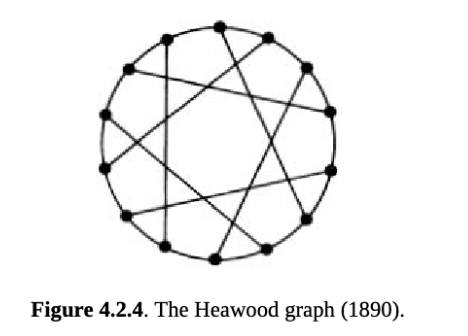
\includegraphics[width=0.35\linewidth]{heawood-graph.png} \\
	\textbf{Snark}: 3-regular graph with edge chromatic number 4. A snark has no Hamiltonian cycle. \\
	\textbf{Heawood Graph}: The unique 6-cage (smallest cubic graph with girth 6). Figure 4.2.4. \\
	\textbf{$k$-regular graph}: a graph where every vertex has degree $k$ \\
	\textbf{Cages}: Smallest cubic graph with girth $g$. \\
	\textbf{Circle} $C_n$: $n$ vertices in a cycle. \\
	\textbf{Wheel} $W_n$: $C_n$ plus one vertex adjacent to all vertices in the cycle. \\
	\textbf{Subgraph}: a graph $H$ is a subgraph of $G$ if $V(H) \subseteq V(G)$ and $E(H) \subseteq E(G)$. \\
	\textbf{Proper Subgraph}: a graph $H$ is a proper subgraph of $G$ if $H \ne G$. \\
	\textbf{Components}: disconnected graphs, islands are the components. \\
	\textbf{Induced Subgraph}: Subgraph of $G$ where $W \subseteq V$ with every edge $E$ that has both endpoints in $W$. \\
	\textbf{Isomorphic Graph}: $G_1$ and $G_2$ are isomorphic if $p = |V(G_1)| = |V(G_2)|$ and the vertices of $G_1$ and $G_2$ can be relabelled as 1, $\dots, p$ so that $ij \in E(G_1) \iff ij \in E(G_2)$. \\
	\textbf{Theorem}: If $G_1$ and $G_2$ are isomorphic, then $G_1$ and $G_2$ have the same number of vertices, edges, and degree sequence. \\

	\textbf{Infinite Lattice Graph $L_2$}: vertices are all points in a plane whose coordinates are both itnegers, and two vertices are adjacent if they have geometric distance equal to one. \\

	\section{Counting}
	\textbf{Problem.} \textit{How many subgraphs isomorphic to $K_{1,3}$ are in $K_n$?} Choose 4 vertices from $n$ vertices: $nC4$. Every choice has 4 possibilities to form $K_{1,3}$ subgraph. So answer is $4 nC4$. \\
	\textbf{Problem.} \textit{How many 1-factors are there in $K_{2h}$?} There are $2h-1$ first pairs, $2h-3$ second pairs, so $(2h-1)(2h-3)(2h-5) \cdots (3)(1)$ possible pair combinations. Then multiply and divide by $(2h-2)(2h-4) \cdots (4)(2) = 2^{h-1}(h-1)!$ to get $(2h-1)!/(2^{h-1}(h-1)!)$. \\
	% giving up on this one since it's too long and requires an identity with $e$.
	% \textbf{Problem.} \textit{How many 1-factors are in the graph $G = K_{n,n}$ minus a 1-factor?} Also called the derangements of $n$ objects. Let $D_n$ denote the number of derangements. Clearly, $D_1 = 0$ and $D_2 = 1$. Denote a node $a$ to be coloured red, and $a'$ to be its blue counterpart. Then the number of 1-factors containing $ij'$ and $ji'$ are $D_{n-1}$, so $(n-1)D_{n-2}$ possibilities. And 1-factors containing $ij'$ but not $ji'$ are $D_{n-1}$ possibilities, so $(n-1)D_{n-1}$ possiblities. Then $D_n = (n-1)(D_{n-1} + D_{n-2}) \Rightarrow D_n - nD_{n-1} = -(D_{n-1} - (n-1)D_{n-2})$. Substiting $n := n-1$, which is $D_{n-1} - (n-1)D_{n-2} = -(D_{n-2} - (n-2)D_{n-3})$, we get $D_n - nD_{n-1} = (-1)^2(D_{n-2} - (n-2)D_{n-3})$ and repetition will get $D_{n} - nD_{n-1} = (-1)n^{-2}(D_2 - D_1) = (-1)^{n-2} = (-1)^n$ so we have $D_n = nD_{n-1} + (-1)^n$. Dividing by $n! = (n-1)!n, we get$
	\textbf{Problem.} \textit{Problem. How many 1-factors are in the graph $G = K_{n,n}$ minus a 1-factor?}
	$D_n = n!(1/2! - 1/3! + \cdots + (-1)^{n-1}/(n-1)! + (-1)^n/n!)$
	\section{Spanning Trees}
	\textbf{Theorem 5.2.1.} The number of spanning trees in $K_n$ is $s(K_n) = n^{n-2}$.
	\textbf{Constructing a sequence}:
	\begin{enumerate}
		\item Identify all the leaves (vertices with degree 1) currently in the tree.
		\item Select the leaf with the smallest label.
		\item Find the unique vertex adjacent to this leaf and add that neighbor's label to the sequence.
		\item Remove the selected leaf and its incident edge from the tree.
		\item Repeat steps 1 through 4 until only two vertices and one edge remain.
		\item The resulting list of recorded labels is the sequence of length $n-2$.
	\end{enumerate}
	\textbf{Theorem.} The number of spanning trees in a complete bipartite graph $K_{m,n}$ is $s(K_{m,n} = m^{n-1}n^{m-1})$ \\
	% \textbf{Proof.} For the unique case $K_{3, n}$: There are three blue vertices $a, b,$ and $c$, and $n$ red vertices.

	% In any spanning tree of $K_{3, n}$ either each of the pairs $\{a, b\}$, $\{a, c\}$, and $\{b, c\}$ has distance two as in Figure 5.3.2, or one of the pairs has distance four as in Figure 5.3.3. \\
	% 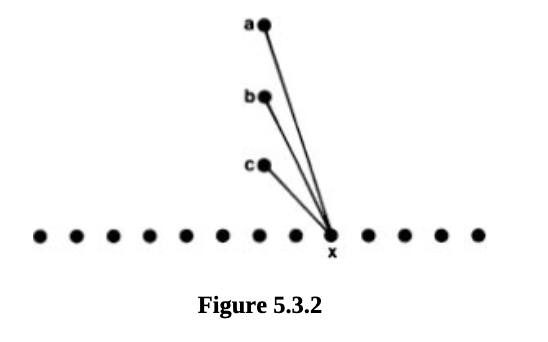
\includegraphics[width=0.45\linewidth]{figure-5.3.2.png} 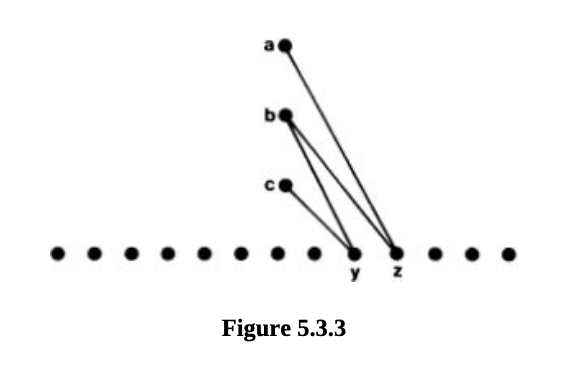
\includegraphics[width=0.5\linewidth]{figure-5.3.3.png} \\
	% We count the number of spanning trees in Figure 5.3.2. There are $n$ ways to choose the vertex $x$. For each of the remaining $n-1$ red vertices, there are three possibilities. Each is either adjacent to $a$, to $b$, or to $c$. Thus there are $n 3^{n-1}$ spanning trees with each pair $\{a, b\}$, $\{a, c\}$, and $\{b, c\}$ having distance two.

	% For Figure 5.3.3, if the points $y$ and $z$ are chosen, there are six possibilities for the path of length four, since there are three ways to choose the center point (in the figure, $b$), and $y$ and $z$ can be interchanged. There are $\binom{n}{2} = \frac{n(n-1)}{2}$ ways to choose the pair $y$ and $z$, and for each of the remaining $n-2$ red vertices there are again three possibilities. Hence for Figure 5.3.3 there are $6 \frac{n(n-1)}{2} 3^{n-2} = n(n-1) 3^{n-1}$ different spanning trees. So the total number is $n 3^{n-1} + n(n-1) 3^{n-1} = n^2 3^{n-1}$.

	\section{Magic Graphs}
	\textbf{Magic Graph:} $G$ is magic if the edges of $G$ can be labeled by the numbers $1,2,3,\dots, q$ so that the sum of the labels of all the edges incident with any vertex is the same. \\
	\textbf{Anti Graph:} $G$ is antimagic if no 2 vertices have the same sum.
	\textbf{Theorem 6.1.1.} $K_{n,n}$ is magic for $n \ne 2$. \\
	\textbf{Theorem 6.1.2.} If a bipartite graph $G$ is decomposable into two Hamilton cycles, then $G$ is magic. \\
	\textbf{Theorem 6.1.3.} If a graph $G$ is decomposable into two magic spanning subgraphs $G_1$ and $G_2$ where $G_2$ is regular, then $G$ is magic. \\
	\textbf{Theorem:} sum of labels at any given vertex is different from the sum of the labels at any other vertex \\
	\textbf{Conjecture:} Every connected graph different from $K_2$ is antimagic.

	\section{Graceful graphs/trees}
	\textbf{Graceful Graphs:} A tree is graceful if the label on any edge equals the difference between the labels of the two endpoints. Vertices must be labled $1,2,3,\dots,n$ and edges $1,2,3,\dots,n-1$. \\
	\textbf{Theorem 6.1.4.} if a tree $T$ with $n$ edges is graceful, then the complete graph $K_{2n+1}$ is decomposable into $2n+1$ trees, each isomorphic to the given tree $T$. \\
	\textbf{Consecutive Labeling:} tree $T$ is consecutive if its vertices and edges can be labeled with the numbers $1,2,3,\dots, 2n-1$ s.t. every edge label equals diff of labels of its two incident vertices. \\
	\textbf{Theorem 6.1.5.} if a tree $T$ is graceful, then $T$ is consecutive. \textbf{Proof:} relable all vertices $k$ with $2k-1$ and recalculate edges to get a consecutive graph.

	\section{Conservative Graphs}
	\textbf{Semantics:} Labels on a directed graph add when label is on an in edge, and subtract on an out edge \\
	\textbf{Conservative Graph/Kirchhoff's Current Law:} In a directed labeling of a conservative graph, the sum of the incoming labels is equal to the sum of the outgoing labels at each vertex. \\
	\textbf{Theorem 6.2.1.} If $G$ is decomposable into two Hamilton cycles, then $G$ is conservative and strongly conservative. \\
	\textbf{Kirchhoff's Global Current Law:} If $G$ is a labeled, directed graph such that Kirchhoff's Current Law holds at every vertex of $G$ except a particular vertex $a$, then Kirchhoff's Current Law also holds at vertex $a$. \\
	\textbf{Strongly Conservative:} A graph $G$ is strongly conservative if for every number $h$ there exists a directed labeling of the edges of $G$ with numbers $h+1, h+2, \dots, h+|E|$ s.t. Kirchhoff's Current Law holds at every vertex. \\
	\textbf{Theorem 6.2.3.} If $G$ is decomposable into two subgraphs $H_1$ and $H_2$, and if $H_1$ is conservative, and $H_2$ is strongly conservative, then $G$ is conservative. Moreover, if both $H_1$ and $H_2$ are strongly conservative, then $G$ is strongly conservative. \\
	\textbf{Theorem 6.2.4.} If graph $G$ has $n$ vertices with $n$ odd, and $G$ is decomposable into three Hamilton cycles, then $G$ is strongly conservative. \\
	\textbf{Theorem 6.2.5.} If $n$ is odd, $n \ge 5$, then $K_n$ is conservative. \\
	\textbf{Theorem 6.2.6.} For $n \ge 3$, the wheel with $n$ spokes, $W_n$, is conservative. \\
	\textbf{Theorem 6.2.7.} If $n$ is even, $n \ge 4$, then $K_n$ is conservative. \\

	\section{Spanning Tree Algorithms}
	\textbf{Algo for unweighted graph:}
	\begin{enumerate}
		\item Start with any edge $e$ and add it and its endpoints to the tree
		\item Check whether the neighbors of the vertices in the tree are in the tree. If not, add them and their incident edges to the tree.
		\item Repeat until all vertices are in the tree.
	\end{enumerate}
	\textbf{Algo for weighted graph (Kruskal's):}
	\begin{enumerate}
		\item Select the edge with the smallest weight. If it does not create a cycle, add it to the tree.
		\item Repeat until all vertices are in the tree.
	\end{enumerate}
	\section{Matching}
	\textbf{Matching}: A matching in a bipartite graph is a subgraph that is regular with degree 1. \\
	\textbf{M-Alternating Path}: Given a matching M, an M-alternating path is a path that alternates between edges in M and edges not in M. \\
	\textbf{M-Augmenting Path}: An M-alternating path that joins two unmatched vertices. \\
	\textbf{Theorem}: A matching M is maximal if and only if there are no M-augmenting paths. \\
	\textbf{Hungarian Algorithm}: A greedy algorithm to find a maximal matching in a bipartite graph.
	\begin{enumerate}
		\item Start with any matching M.
		\item Find an M-augmenting path.
		\item Add the edges in the M-augmenting path to the matching and remove the edges that are in the path from the matching.
		\item Repeat until no M-augmenting paths are found.
	\end{enumerate}
	\section{Binary Trees \& Prefix Codes}
	\textbf{Rooted Tree}: A directed tree with a root node with indegree 1. \\
	\textbf{Binary Tree}: A rooted tree where every vertex has outdegree at most 2. \\
	\textbf{Alphabet}: A finite set of symbols. \\
	\textbf{Code}: A set of sequences of symbols from an alphabet \\
	\textbf{Prefix Code}: A code where no codeword is a prefix of another cdeword. \\
	\textbf{Prefix Code Tree}: A binary tree with left edges labeled 0 and right edges labeled 1, paths from the root to a leaf form the codewords in a prefix code. \\
	\textbf{Weighted Binary Tree}: A binary tree where each leaf is assigned a weight equal to how often the symbol appears in the message. The weight of the tree is the sum of the weights of the leaves each multiplied by the depth of the leaf. Minimizing the weight of the tree is equivalent to finding a minimal encoding tree. \\
	\textbf{Multiset}: A set where elements can appear multiple times. Given a Multiset of weights $M$, a \textbf{minimum weight binary tree} is a binary tree with the minimum weight that encodes the symbols in $M$. \\
	\textbf{Huffman Algorithm}: A greedy algorithm to find a minimum weight binary tree.
	\begin{enumerate}
		\item Select two smallest weights $w_1, w_2$ in $M$. Create parent labeled $w_1 + w_2$ with leaves $w_1, w_2$. Cross out $w_1, w_2$ in $M$; add $w_1 + w_2$ to $M$.
		\item Repeat: Select two smallest in $M$. If one labels an existing vertex (subtree root), attach that subtree; else create new leaves. Label new vertex with sum, cross out the two in $M$, replace with their sum.
		\item Stop when $|M| = 1$; $T$ is the minimum-weight binary tree.
	\end{enumerate}

	\section{Planar Graphs}
	\textbf{Planar Graph}: A graph that can be drawn on a plane without any edges crossing. \\
	\textbf{Face}: A region of the plane that is bounded by edges. \\
	\textbf{Plane Drawing}: A drawing of the graph in the plane with no crossings. \\
	\textbf{Outside Triangle}: The triangle representing the outside of a shape. \\
	\textbf{Convex}: A region in a plane drawing of a planar graph s.t. whenever any two points on the boundary of or in the region are connected by a straight line segment, the straight line segment lies entirely inside the region. \\
	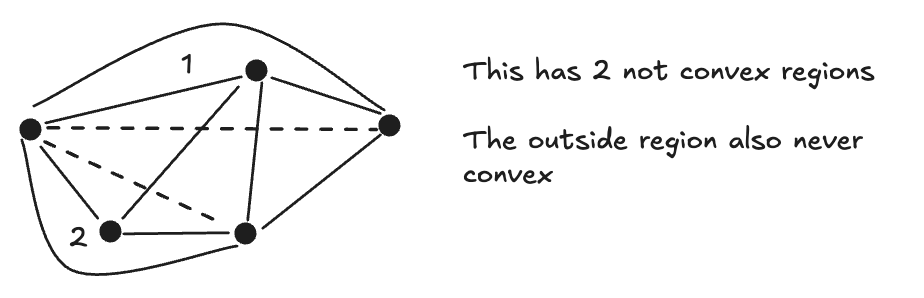
\includegraphics[width=0.6\linewidth]{figure-8.4.2.png} \\
	\textbf{Coin graph}: a graph where every vertex is a coin and two vertices are adjacent iff the coins touch. \\
	\textbf{Penny graph}: A coin graph where every coin is the same size. \\

	\textbf{Theorem 8.1.1 (Euler's Polyhedral Formula)}: If $G$ is a connected planar graph with $p$ vertices, $q$ edges, and $r$ regions/faces, then $p - q + r = 2$. Proof uses induction on number of cycles in graph.\\
	\textbf{Maximal Planar Graph}: A graph is maximal planar if adding any edge would create a non-planar graph. \\
	\textbf{Theorem 8.1.2}: If $G$ is a maximal planar graph with $p$ vertices and $p \geq 3$, then $q = 3p - 6$. \\
	\textbf{Theorem 8.1.4/6}: The graphs $K_5$ and $K_{3,3}$ are not planar. \\
	\textbf{Theorem 8.1.5}: If $G$ is a planar bipartite graph with $p$ vertices and $p \geq 3$, then $q \leq 2p - 4$. \\
	\textbf{Theorem 8.1.7}: Every planar graph has at least one vertex with degree $\leq 5$. \\
	\textbf{Theorem 8.1.8}: Suppose $G$ is a planar graph with $p \geq 4$. Let $p_i$ be the number of vertices of degree $i$. Then $3p_3 + 2p_4 + p_5 = 12 + p_7 + 2p_8 + 3p_9 + \cdots$. \\
	\textbf{Theorem 8.4.1. (Wagner).} Every planar graph has a plane drawing where every edge is a straight line. If such a drawing exists, $G$ is \textbf{stretchable}. \\
	\textbf{Theorem 8.4.2. (Koebe).} Every planar graph is a coin graph.

	\section{Country Coloring}
	\textbf{Lune}: A region of a plane drawing of a multigraph containing two edges. \\
	\textbf{Map}: A plane drawing of a connected, bridgeless, planar multigraph. \\
	\textbf{Normal Map}: A map that is cubic. \\
	\textbf{Country}: A region of a map. Adjacent countries share an edge. \\
	\textbf{Empire ($m$-pire)}: A collection of $m$ disjoint countries is an empire (or $m$-pire). Two empires are adjacent if they share a common boundary edge. \\
	\textbf{Map Coloring Problem}: Color the countries of a map using the fewest colors such that no two adjacent countries have the same color. \\
	\textbf{Dual}: A multigraph $G(M)$ is a dual of a map $M$ if the vertices of $G(M)$ are the faces of $M$, and two vertices of $G(M)$ are adjacent if and only if the corresponding faces of $M$ share an edge. This multigraph is planar. $G(G(M)) = M$ for $p \ge 4$. \\
	\textbf{Theorem 8.2.1/3 (Tait)} If a normal map has a coloring of the countries using $4$ colors, then the edges of the map can be properly colored using $3$ colors. Vice versa is also true. \\
	\textbf{Lemma 8.2.2}: Given a finite number of simple closed curves (cycles) in the plane, the regions defined by those curves are colorable with $2$ colors. \\
	\textbf{Theorem 8.2.4/5}: If in a normal map the edges are properly colored using $3$ colors, then the vertices can be labeled black or white so that around any given country, the number of black vertices minus the number of white vertices is always a multiple of $3$. Vice versa is also true. \\
	\textbf{Theorem 8.2.6 (Four Color Theorem)}: Every normal map can be colored using $4$ colors. \\
	\textbf{Theorem 8.2.7}: In every planar cubic bridgeless graph, the edges are properly colored using $3$ colors. Equivalent to Four Color Theorem. \\
	If $D$ is a plane drawing of a maximal planar graph with at least $4$ vertices, then $G(D)$ is a normal map. \\
	\textbf{Theorem 8.2.8 (Dual version of Four Color Theorem)}: The vertices of every maximal planar graph with at least $4$ vertices can be can be colored with at most $4$ colors. \\
	\textbf{Theorem 8.2.9}: The vertices of every planar graph can be colored with at most $4$ colors. \\
	\textbf{Theorem.} If $M$ is maximal planar map, $p \ge 4$, then $G(M)$ is a normal map.
	\textbf{Lemma 8.3.1}:No map in the plane has five mutually adjacent countries. Proof: If it did, the dual would contain a subgraph isomorphic to $K_5$, which is not planar. \\
	\textbf{Five Color Theorem}: The countries of every normal map in the plane can be colored with five colors. \\
	\textbf{Theorem 9.3.1 (Heawood, 1890).} Every $2$-pire map can be colored with $12$ colors, and there exist $2$-pire maps that require $12$ colors. \\
	\textbf{Theorem 9.3.2 (Heawood).} Every $m$-pire map can be colored with $6m$ colors. \\
	\textbf{Theorem 9.3.3 (Heawood, Jackson, Ringel).} For every $m > 1$, there exists a map in the plane with $6m$ mutually adjacent $m$-pires. \\
	\textbf{Problem.} Find a 2-pire map in the plane with the largest number of 2-pires such that every pair of 2-pires is adjacent twice.
	\textbf{Solution.} Let $n$ be the number of $2$-pires in the map. Then the dual of the map has $2n$ vertices and $2\binom{n}{2} = n(n-1)$ edges. We know by **Theorem 8.1.3** that $q \leq 3p - 6$, so in this instance $n(n-1) \leq 6n-6 \Rightarrow n^2 - 7n + 6 \leq 0 \Rightarrow (n-1)(n-6) \leq 0$. Since $n-1$ is positive, $n-6 \leq 0$, hence $n \leq 6$. \\
	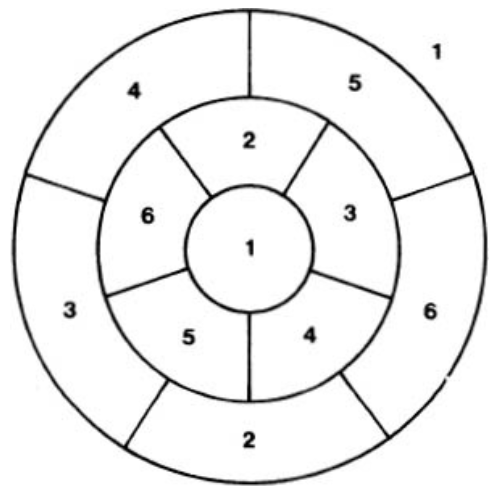
\includegraphics[width=0.25\linewidth]{empire-problem1.png}
	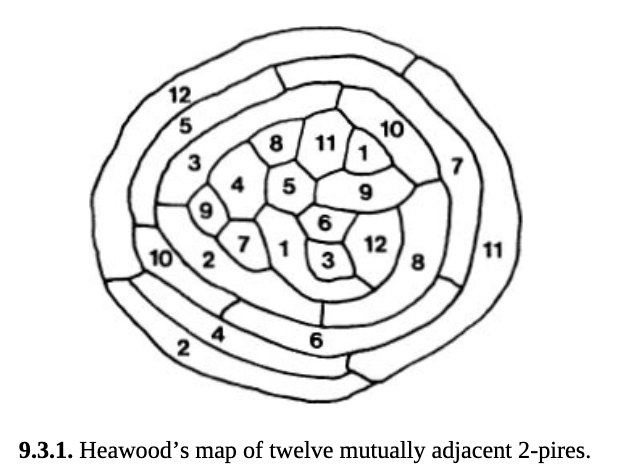
\includegraphics[width=0.35\linewidth]{heawood-twelve.png}
	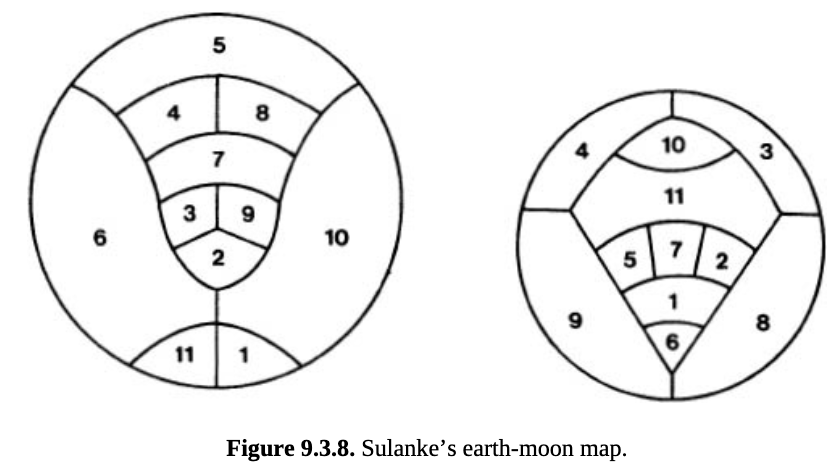
\includegraphics[width=0.35\linewidth]{earth-moon.png} \\
	\textbf{Earth-Moon Problem.} Disconnected places called Earth and Moon. What is the smallest number $k_2$ of colors so that every earth-moon map can be colored by $k_2$ colors? Each $2$-pire must have country on both earth and moon. \\
	\textbf{Solution.} Find a 2-pire map in the plane with the largest number of 2-pires such that every pair of 2-pires is adjacent twice. See above left most figure. \\
	\textbf{Problem.} Find a 2-pire map in the plane with the largest number of 2-pires such that every pair of 2-pires is adjacent twice. \textbf{Solution.} See fig-59.

	\section{Measuring Closeness to Planarity}
	\textbf{Subdivision:} graph $G$ is a subdivision of $H$ if $G$ is $H$ with some vertices of degree 2 added. All graphs are subdivisions of themselves. \\
	\textbf{Theorem.} If $G$ is not planar, then a subdivision of $G$ is not planar. \\
	\textbf{Theorem 9.1.1.} If a graph $G$ contains a subgraph that is a subdivision of $K_{5}$ or of $K_{3,3}$, then $G$ is not planar. \\
	\textbf{Theorem.} Assume that $G$ is a graph with the property that $G$ is not planar, and for every edge $e$ of $G$, the graph $G-e$ is planar. Then $G$ is either a subdivision of $K_{5}$ or a subdivision of $K_{3,3}$. \\
	\textbf{Theorem 9.1.2.} (Kuratowski). If $G$ is a nonplanar graph, then $G$ contains a subgraph that is a subdivision of $K_{5}$ or of $K_{3,3}$. \\
	\textbf{Simple Drawing}: A simple drawing of a graph in the plane is a drawing in which:
	\begin{enumerate}
		\item[a)] any two distinct edges have at most one crossing.
		\item[b)] any two edges incident with the same vertex do not cross.
		\item[c)] no three edges cross in a common point.
	\end{enumerate}
	\textbf{Multiple Crossing:} If more than 2 edges cross at the same point, it's called a multiple crossing. \\
	\textbf{Crossing Number:} There exists a drawing of $G$ that has the minimum number of crossings such that $G$ also has no multiple crossings. That min number is called crossing number, denoted $cr(G)$. Such a drawing is always a simple drawing. Crossing number of all planar graphs is 0. $cr(K_{5})=1$ and $cr(K_{3,3})=1$ \\
	\textbf{Theorem 9.1.3.} Every simple drawing of $K_{4}$ in the plane has either zero or one crossing. \\
	\textbf{Theorem 9.1.4.} The crossing number of $K_{6}$ is $cr(K_{6})=3$. \\
	\textbf{Theorem.} For a complete graph $K_{n}$, the following inequality holds: $cr(K_{n}) \le 1/4 \left\lfloor n/2\right\rfloor\left\lfloor (n-1)/2\right\rfloor \left\lfloor (n-2)/2\right\rfloor\left\lfloor (n-3)/2\right\rfloor$ \\
	\textbf{Theorem.} For a complete bipartite graph $K_{m,n}$, we have: $cr(K_{2t,2s}) \le t(t-1)s(s-1)$, $cr(K_{2t+1,2s+1}) \le t^{2}s^{2}$, $cr(K_{2t+1,2s}) \le t^{2}s(s-1)$ \\
	\textbf{Theorem 9.1.5.} The crossing number of $K_{m,n}$ satisfies the inequality $cr(K_{m,n}) \le \lfloor m/2 \rfloor \lfloor (m-1)/2 \rfloor \lfloor n/2 \rfloor \lfloor (n-1)/2 \rfloor$ \\
	\textbf{Theorem 9.1.6.} The crossing number of $K_{3,n}$ is $cr(K_{3,n}) = \lfloor n/2 \rfloor \lfloor (n-1)/2 \rfloor$ \\
	\textbf{Theorem 9.1.7.} The crossing number of $K_{4,n}$ is $cr(K_{4,n}) = 2 \lfloor n/2 \rfloor \lfloor (n-1)/2 \rfloor$ \\

	\section{Thickness and Splitting Number}
	\textbf{Thickness} $\theta(G)$: Minimum $t$ such that $G = H_1 \cup \cdots \cup H_t$ where each $H_i$ is planar (union of edge-disjoint planar subgraphs); no decomposition into fewer than $t$ planar subgraphs exists. \\
	\textbf{Theorem 9.2.1.} $p,q$ vertices/edges: $\theta(G)\ge q/(3p-6)$. \\
	\textbf{Theorem 9.2.2.} $G$ bipartite, $p,q$ as above: $\theta(G)\ge q/(2p-4)$. \\
	\textbf{Theorem 9.2.3.} $\theta(K_n)=\lfloor(n+7)/6\rfloor$ for $n\neq 9,10$; $\theta(K_n)=3$ for $n\in\{9,10\}$. (9.2.1, $n\ge 3$: $\theta(K_n)\ge\lceil n(n-1)/(6(n-2))\rceil=\lfloor(n+7)/6\rfloor$.) \\
	\textbf{Partial ($K_{m,n}$).} $\theta(K_{m,n})\ge mn/(2(m+n-2))$; if $mn$ even, $\theta(K_{m,n})=\lceil mn/(2(m+n-2))\rceil$ (9.2.2). \\
	\textbf{Identifying vertices}: Let $u,v \in V(G)$. Build $G'$ by replacing $u$ and $v$ with one new vertex $w$, with $w$ adjacent to every vertex that was adjacent to $u$ or $v$ in $G$. This is \textbf{identifying} $u$ and $v$. (Often the two vertices are denoted by the same symbol before identifying.) \\
	\textbf{Splitting a vertex}: Replace $w \in V(G)$ by two vertices $u$ and $v$ so $u$ is adjacent to some of $w$'s former neighbors and $v$ to the rest; $u$ and $v$ need not be adjacent. \textbf{Splitting} and \textbf{identifying} are opposite operations. \\
	\textbf{Splitting number} $\sigma(G)$: Smallest $K$ such that $G$ can be obtained from a planar graph $H$ by $K$ vertex identifications; equivalently, the minimum number of vertex splittings needed to turn $G$ into a planar graph $H$. Such an $H$ is a \textbf{planar splitting} of $G$. \\
	\textbf{Examples:} $\sigma(K_5)=1$, $\sigma(K_6)=2$, $\sigma(K_7)=3$, $\sigma(K_8)=4$, $\sigma(K_9)=6$. \\
	\textbf{Theorem 9.2.4 (Hartsfield, Jackson, Ringel).} $n\le 10$: $\sigma(K_n)=\lceil(n-3)(n-4)/6\rceil$. \\
	\textbf{Theorem 9.2.5 (Jackson, Ringel).} $m,n\ge 2$: $\sigma(K_{m,n})=\lceil(m-2)(n-2)/2\rceil$. \\
	\textbf{Inequality:} With $p = |V|$, $q = |E|$, $(q - 3p + 6)/3 \le \sigma(G)$.

	\section{Rotations on Graphs}
	\textbf{Rotation of G}: A rotation ($\rho$) of $G$ is a coloration of vertices of some cubic graph $G$ such that each vertex is black or white. Black vertices indicate clockwise and white vertices indicate counterclockwise. A graph $G$ has $2^{|V|}$ possible rotations.\\
	\textbf{Rotations Induce Curcuits}: A rotation $\rho$ induces cicuits in a graph: Start at an edge and travel along it in one of the two directions. If you hit a black vertex, turn clockwise until you find an edge to continue walking along, and counterclockwise if you hit a white vertex. Continue until you return to the same starting edge and direction. NOTE, circuits induced by rotations may have repeated vertices and edges used in both directions.\\
	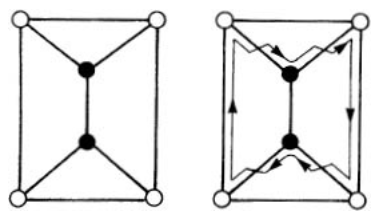
\includegraphics[width=0.35\linewidth]{figure-10.1.2.png}
	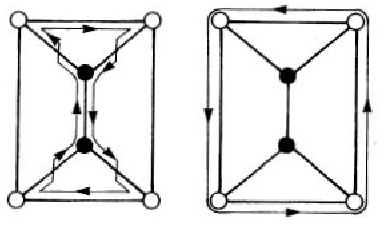
\includegraphics[width=0.35\linewidth]{figure-10.1.3.png} 	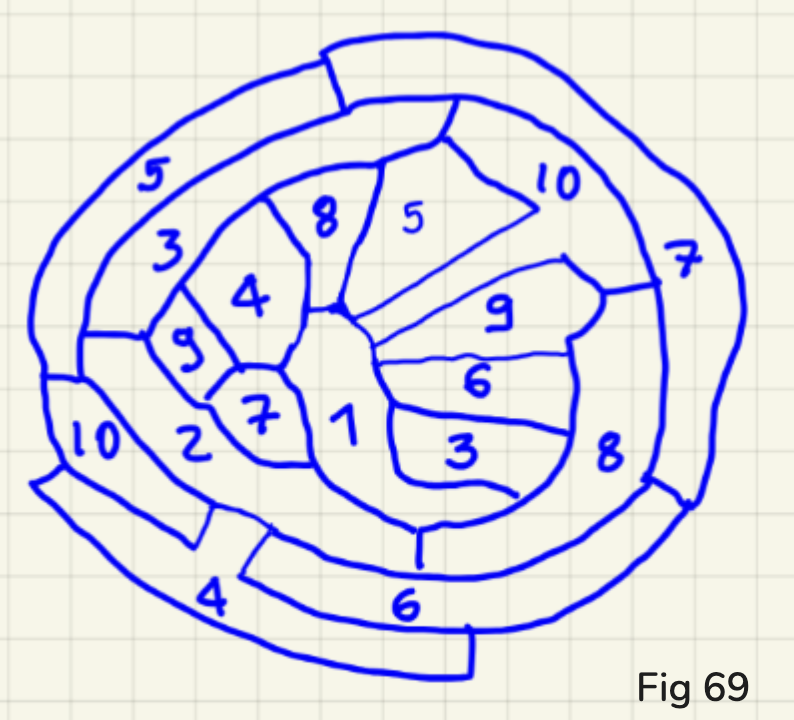
\includegraphics[width=0.25\linewidth]{fig-59.png} \\
	\textbf{Definition $r(\rho)$}: A rotation $\rho$ partitions $G$ into $r(\rho)$ circuits. Different rotations $\rho$ may induce different numbers of circuits. \\
	\textbf{Circular Rotation}: A rotation $\rho$ is circular if it induces a single circuit. \\
	\textbf{Scheme}: A listing of each vertex in a graph where each vertex is numbered and assigned a list of vertices it is adjacent to. Esentially an adjacency list of a graph.\\
	\textbf{Rotation of Vertices}: A rotation for a particular vertex is an ordered cyclic listing of vertices adjacent to that vertex. Example above shows how that listing can be used to describe a rotation. \\
	\textbf{Theorem 10.1.1}: If vertex $v$ has degree $d$, then there are $(d-1)!$ rotations of $v$. \\
	\textbf{Deriving circuits from schemes}:
	\begin{enumerate}
		\item Pick edge $uv$
		\item Scheme of $v$ is $v: \dots ux \dots$. Pick $x$ to be next.
		\item Continue until $uv$ is reached again.
	\end{enumerate}
	\textbf{Theorem 10.1.2}: Given a connected graph with $p$ vertices and $q$ edges, and a rotation $\rho$ which induces $r(\rho)$ circuits, the inequality $p-q+r(\rho) \leq 2$ holds. Furthermore, the alternating sum $p-q+r(\rho)$ is even. \\
	The proof for this uses induction on the number of cycles in the graph. \\
	\section{Planar Graphs With Rotations}
	\textbf{Definition} If $G$ is connected, and there exists a rotation $\rho$ of $G$ such that $p-q+r(\rho) = 2$, then $\rho$ is a \textbf{planar rotation} of $G$ and $G$ is a \textbf{connected planar graph}. If $G$ is not connected, consider the connected subgraphs of $G$. If each subgraph satisfies the above conditions, the entire graph is \textbf{planar}. \\
	\textbf{Theorem 10.2.1}: If $G$ has a bridge, then for any rotation $\rho$ of $G$, the bridge occurs in both directions in one curcit induced by $\rho$. \\
	Proof idea: A circuit starting on one side of the bridge and crossing it must come back since its closed, so it must cross the bridge in both directions. \\
	\textbf{Theorem 10.2.2}: If $H$ is a subgraph of planar graph $G$, then $H$ is planar. \\
	Many theorems in this section are repeats of planar graph theorems, but they use rotations to prove them, for example:
	\textbf{Theorem 10.2.3}: The complete bipartite graph $K_{3,3}$ is not planar. \\
	Proof: If $K_{3,3}$ were planar, then it would have a rotation $\rho$ such that $p-q+r(\rho) = 2$. However, $K_{3,3}$ has 6 vertices and 9 edges, so $p-q+r(\rho) = 6-9+r(\rho) = 2$, so $r(\rho) = 5$, which would mean that the average circuit length is $(9*2)/5 = 3.6$ since each edge is used twice (both directions), but the shortest circuit length is 4, so $K_{3,3}$ cannot be planar. \\
	\textbf{Theorem 10.2.5}: A maximal planar graph $G$ with three or more vertices is connected and has no bridge. \\
	% Proof outline: Suppose $G$ is not connected, we can add an edge to connect two components without creating a crossing, so $G$ was not maximal. Suppose $G$ has a bridge, we can add an edge such that one circuit containing the bridge becomes two circuits, so by the planar rotation definition, adding this edge keeps the graph planar, so$G$ was not maximal. \\
	\textbf{Theorem 10.2.6}: Every planar rotation $\rho$ of a maximal planar graph $G$ has the property that every circuit induced by $\rho$ has length 3. \\
	% Proof outline: Case that length $\geq 5$: In a circuit of length at least 5, at least one pair of vertices is not adjacent, otherwise the graph contains a subgraph isomorphic to $K_5$, which is not planar. create an edge between these two vertices, thereby creating two circuits from one and adding an edge, so this new graph is therefore planar by the planar rotation definition, meaning $G$ was not maximal.\\ Case that length $= 4$: In a circuit of length 4, if any two vertices are not adjacent, do the same as previous case. Otherwise, create a new vertex and connect it to all 4 vertices in the cycle, thereby creating 4 circuits from one and adding 4 edges and 1 vertex, so this new graph is therefore planar by the planar rotation definition, meaning $G$ was not maximal.\\
	\textbf{Theorem 10.2.9}: A connected graph that can be drawn in the plane with no crossings has a planar rotation. \textbf{Proof}: Take the plane drawing and assign all vertices black, resulting in a circuit for each region, so by the planar rotation definition, the graph has a planar rotation. \\

	\section{Genus of a Graph}
	\textbf{Orientable Surface of Genus $g$ or $S_g$}: Sphere is $S_0$ (no handles); torus $S_1$ (one handle); in general attach $g$ handles to a sphere. Planar graphs embed in $S_0$ (sphere = plane $+$ point at $\infty$). \\
	\textbf{Embeddable}: $G$ embeds in $S_g$ if it can be drawn on $S_g$ with no edge crossings. If $G$ embeds in $S_g$, it embeds in $S_{g+1}$. \\
	\textbf{Genus} $\gamma(G)$: Minimal $g$ such that $G$ embeds in $S_g$. Then $\gamma(G)=g$ means $G$ embeds in $S_g$ but not in $S_{g-1}$. Planar $\Leftrightarrow$ $\gamma(G)=0$. \\
	\textbf{Genus (Alternative Definition)}: For connected $G$ and maximal $\rho$, $p-q+r(\rho)=2-2\gamma(G)$ ($g$ nonnegative integer; agrees with planar rotation when $\gamma=0$). E.g.\ $K_7$: $p=7$, $q=21$, $r(\rho)=14$ $\Rightarrow$ $7-21+14=0=2-2(1)$ so $\gamma(K_7)=1$; similarly $\gamma(K_{4,4})=1$. \\
	\textbf{Mapping onto a Rectangle}: Proof of $\gamma(K_5)=\gamma(K_{3,3})=\gamma(K_7)=\gamma(K_{4,4})=1$ (torus) \\
	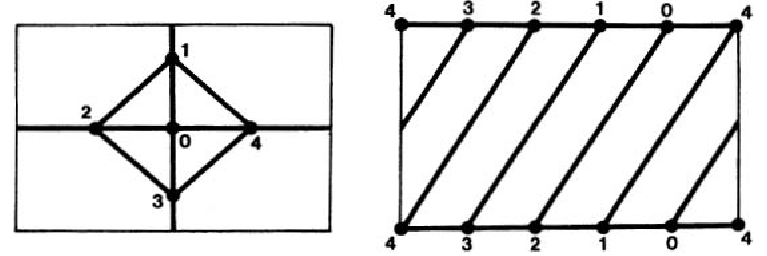
\includegraphics[width=0.45\linewidth]{figure-10.3.4.png}
	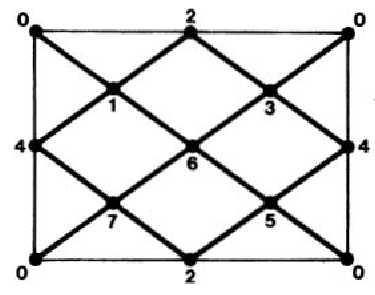
\includegraphics[width=0.22\linewidth]{figure-10.3.6.png}
	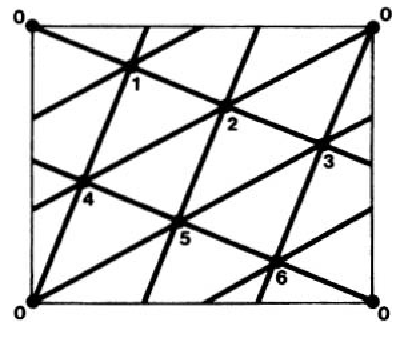
\includegraphics[width=0.22\linewidth]{figure-10.3.7.png} \\
	\textbf{Maximal rotation}: $\rho$ is maximal if $r(\rho)$ is as large as possible; when a planar rotation is maximal (Thm 10.1.2: $p-q+r(\rho)\le 2$, even). \\
	\textbf{Theorem 10.3.1}: If every circuit induced by $\rho$ has length three, then $\rho$ is a maximal rotation. \\
	\textbf{Theorem 10.3.2}: In a bipartite $G$, if every circuit induced by $\rho$ has length four, then $\rho$ is maximal. \\
	\textbf{Theorem 10.3.3--10.3.4 (Ringel)}: $\gamma(K_{m,n})=\lceil (m-2)(n-2)/4 \rceil$ for $m,n\ge 2$. (Proof idea: bipartite $\Rightarrow$ shortest induced circuit $\ge 4$, so $2q\ge 4r(\rho)$; combine with $p-q+r(\rho)=2-2g$.) \\
	\textbf{Rule $\Delta^*$}: If row $i$ is $\ldots,j,k,\ldots$, then row $k$ is $\ldots,i,j,\ldots$ $\Rightarrow$ every induced circuit has length three (triangular faces). \\
	\textbf{Rule $R^*$}: If row $i$ is $\ldots,j,k,l,\ldots$, then row $k$ is $\ldots,l,i,j,\ldots$. Rules $\Delta^*$ and $R^*$ are equivalent. \\
	\textbf{Note}: $K_8$ has no rotation with all circuits length $3$ since $2q=56$ is not divisible by $3$. \\
	\textbf{Theorem}: Lower bound on $\gamma(K_n)$ from $2q\ge 3r(\rho)$ and $p-q+r(\rho)=2-2g$ for maximal $\rho$. \\
	\textbf{Theorem 10.3.6 (Ringel, Youngs)}: $\gamma(K_n)=\lceil (n-3)(n-4)/12 \rceil$ for $n\ge 3$. \\
	\textbf{Theorem 10.3.7 (Heawood)}: If $G$ is critical with chromatic number $\chi$ and $\gamma(G)\le g$ with $g\ge 1$, then $\chi(G) \le \lfloor (7+\sqrt{48g+1})/2 \rfloor$ (the Heawood number $H(g)$). For $g=0$ this is not Heawood; use the Four Color Theorem instead. \\
	\textbf{Theorem 10.3.8 (Map Color Theorem)}: For every $g\ge 1$, there exists a critical graph $G$ and $\gamma(G) \ge g$ and $\chi (G) = \lfloor (7 + \sqrt{1 + 48g})/2 \rfloor$ \\

\end{multicols*}

\end{document}